% =====================================================================
% Calibration and Efficiency of Uncertainty Estimates in IVIM
% Reconstructed editable LaTeX source (baseline = MRM-submission PDF).
% Built with tectonic: `tectonic manuscript.tex`
% =====================================================================
\documentclass[11pt]{article}
\usepackage[margin=1in]{geometry}
\usepackage{graphicx}
\usepackage{amsmath}
\usepackage{amssymb}
\usepackage{booktabs}
\usepackage[table]{xcolor}
\usepackage{microtype}
\usepackage{setspace}
\usepackage{array}
\usepackage[font=small,labelfont=bf]{caption}
\usepackage[hidelinks]{hyperref}

\graphicspath{{../figures/manuscript/}}

% --- convenience macros (keep notation consistent and error-free) ---
\newcommand{\Dstar}{\ensuremath{D^{*}}}
\newcommand{\Szero}{\ensuremath{S_{0}}}
\newcommand{\x}{\ensuremath{\times}}
\renewcommand{\arraystretch}{1.2}

\setstretch{1.15}
\setlength{\parskip}{0.5em}
\setlength{\parindent}{0pt}

\begin{document}

% ======================= TITLE PAGE =======================
\begin{center}
{\LARGE\bfseries Calibration and Efficiency of Uncertainty Estimates in Intravoxel
Incoherent Motion Imaging: Quantile Intervals, Cross-Paradigm Comparison, and a
Cram\'er--Rao Audit of Amortized Posteriors\par}

\vspace{1em}
{\large\bfseries Avery Karlin, BA\par}
\vspace{0.4em}
{\itshape Department of Applied Physics and Applied Mathematics, Columbia University, New York, NY, USA\par}
{\itshape Department of Computer Science, University of Colorado Boulder, Boulder, CO, USA\par}
\texttt{ak5232@columbia.edu}

\vspace{1em}
Word count (body): $\sim$3,200 \quad$\vert$\quad Figures: 4 \quad$\vert$\quad Tables: 2

\vspace{0.3em}
{\itshape Submitted to Magnetic Resonance in Medicine}
\end{center}

\noindent Corresponding author: Avery Karlin (\texttt{ak5232@columbia.edu}). Conflict of
interest: the author declares no competing interests. Funding: none.

\vspace{1em}

% ======================= ABSTRACT =======================
\section*{Abstract}

\noindent\textbf{Purpose:} To establish whether intravoxel incoherent motion (IVIM)
uncertainty estimates are calibrated across estimation paradigms and amortized neural
posteriors, and to identify diagnostics for miscalibration that aggregate metrics conceal.

\noindent\textbf{Methods:} Two analyses used one biexponential IVIM simulation framework
(24 fitting methods; SNR 10--100; three truths; clinically sparse b-scheme). Aggregate
calibration can be satisfied --- nominal coverage attained --- while an estimator is
pointwise overconfident, intervals too narrow where a parameter is weakly identified. To
expose this, an amortized neural posterior estimator (NPE) was trained and its claimed
precision compared against the Cram\'er--Rao lower bound (CRLB) --- the physical precision
limit --- and a nonlinear least-squares (NLLS) reference, separating claimed from achieved
precision. Robustness was assessed with held-out-b posterior-predictive checks under model
misspecification, acquisition shift, and an open in-vivo dataset. Separately, uncertainty
constructions were compared across classical bootstrap, Bayesian (Laplace, MCMC credible
and quantile intervals), and deep-learning (ensemble, input-perturbation) paradigms, scored
by empirical coverage.

\noindent\textbf{Results:} The NPE passed aggregate coverage yet was pointwise miscalibrated:
claimed \Dstar{} uncertainty was 0.08--0.67\x{} the CRLB floor (overconfident), with achieved
SD 0.02--0.19\x{} (prior-reverting bias), whereas NLLS tracked the floor. On an open in-vivo
dataset, held-out-b coverage collapsed to 0.03 (NLLS 0.90), and $\sim$100\% of points were
overconfident off-scheme. Gaussian credible intervals failed on \Dstar{} (coverage 0.30);
quantile intervals recovered nominal calibration (0.94); deep ensembles captured only
epistemic variance (0.25--0.36), whereas input-perturbation matched the ceiling (0.83--0.94).

\noindent\textbf{Conclusion:} Reliable IVIM uncertainty in the clinical SNR regime benefits
heavily from shape-aware intervals and information-floor benchmarking; aggregate coverage
masks pointwise overconfidence.

\noindent\textbf{Keywords:} IVIM, uncertainty quantification, calibration, simulation-based
inference, Cram\'er--Rao bound, deep learning.

% ======================= INTRODUCTION =======================
\section*{Introduction}

Intravoxel incoherent motion imaging (1) separates tissue diffusion ($D$) from microvascular
pseudodiffusion (\Dstar{}) via a biexponential signal model, with perfusion fraction $f$.
\Dstar{} is notoriously weakly identified: its contribution scales with $f$ (typically
5--20\%) and degrades rapidly at clinical SNR (2--7). Consequently, any point estimate of
\Dstar{} must be accompanied by an honest uncertainty estimate to be clinically usable. Yet
the calibration of IVIM uncertainty has not been systematically established across estimation
paradigms or the increasingly common deep-learning methods, and recent work quantifying
deep-learning IVIM uncertainty (18,19) does not address the cross-paradigm
calibration-and-efficiency question posed here.

Two gaps motivate this work. First, uncertainty can be constructed in many ways ---
bootstrap resampling of a least-squares fit, the curvature of a Bayesian posterior, the
spread of a deep ensemble, or the response of a network to input perturbation --- and it is
not known which constructions yield calibrated intervals on the bounded, skewed parameters
\Dstar{} and $f$. Second, while recent work has introduced simulation-based inference to
diffusion MRI (including generalized frameworks like $\mu$GUIDE (20) and explicit Bayesian
comparisons (21)) alongside concurrent UQ frameworks for IVIM (19), amortized neural
posterior estimators have not been benchmarked against the information-theoretic limit of
the problem.

This work is positioned as a diagnostic contribution rather than an audit of one method.
Relative to recent IVIM and diffusion-MRI uncertainty work, its distinguishing move is to
benchmark a learned posterior against the information floor. Casali et al.\ (19) decompose
supervised IVIM uncertainty into aleatoric and epistemic components but do not test it against
a Cram\'er--Rao information floor; $\mu$GUIDE (20) surfaces parameter degeneracy in a
generalized simulation-based framework without referencing the achievable-precision limit; and
Manzano-Patr\'on et al.\ (21) report simulation-based inference as ``calibrated'' on aggregate
coverage in diffusion MRI --- precisely the aggregate-pass / pointwise-fail mirage this work
dissects pointwise. The portable lesson is methodological: aggregate calibration is necessary
but not sufficient, and floor-referenced, shape-aware auditing is what separates a posterior
that is calibrated on average from one that is trustworthy voxel-by-voxel.

A recurring hazard underlies both gaps: aggregate calibration metrics can be satisfied while
the uncertainty is wrong where it matters. A method can attain nominal marginal coverage by
being overconfident in one region and over-wide in another, the two errors canceling in the
average. Detecting this requires diagnostics sensitive to interval shape and to the
information floor, not merely to average coverage.

We address both gaps within one simulation framework. Part 1 compares uncertainty
constructions across classical, Bayesian, and deep-learning paradigms and identifies which
produce calibrated \Dstar{} and $f$ intervals. Part 2 trains an amortized NPE and audits it
against the CRLB and an NLLS reference, distinguishing claimed from achieved uncertainty. The
transferable contribution is the diagnostic itself: information-floor (CRLB) auditing is a
general check for learned qMRI posteriors --- not specific to IVIM or to one network --- and
the aggregate-passes / pointwise-fails distinction is the portable lesson, because the standard
aggregate checks pass even when the uncertainty is not trustworthy. The amortized NPE studied
here is the worked example through which we exercise that diagnostic, not the object of the
claim.

The scope is correspondingly bounded, and we state it up front: we study a single trained NPE
configuration over one prior and acquisition family, with the normalizing-flow architecture
varied as an ablation. It is the diagnostic, not this particular estimator, that we intend to
generalize.

% ======================= METHODS =======================
\section*{Methods}

\subsection*{Simulation framework (shared)}

Biexponential IVIM signals were simulated as $S(b) = \Szero\,[\,f\cdot\exp(-b\cdot \Dstar) +
(1-f)\cdot\exp(-b\cdot D)\,]$, with $b$ the diffusion weighting (0--1000~s/mm$^2$), $\Szero =
1000$~a.u., and $D, \Dstar$ in $10^{-3}$~mm$^2$/s. Three ground-truth conditions were used:
$(D, \Dstar, f) = (0.7, 30, 0.15)$, $(1.2, 50, 0.10)$, and $(0.5, 20, 0.20)$. Rician noise
was added at SNR $\in \{10, 20, 40, 100\}$. The b-scheme was clinically sparse ($b \in \{0,
10, 20, 30, 50, 100, 200, 400, 600, 800, 1000\}$~s/mm$^2$).

\subsection*{Part 1 --- Uncertainty paradigms and constructions}

Three paradigms were compared. Classical: biexponential and segmented NLLS with residual
bootstrap (8) ($K = 200$). Bayesian (6,9): maximum a posteriori estimation with (a) Laplace
approximation (Gaussian posterior from the central-difference Hessian at the mode), (b) MCMC
with Gaussian credible intervals from the marginal posterior SD, and (c) MCMC with quantile
intervals taken directly from posterior samples. Deep learning: two pre-trained networks
built on the IVIM-NET architecture (16) --- IVIM\_NEToptim (7) and Super\_IVIM\_DC (17) ---
with uncertainty from ensemble-over-retrains (14,15) ($M = 5$; epistemic) and
input-perturbation ($B = 50$; predictive, via Rician re-noising of the reconstructed
signal). All implementations used the OSIPI TF2.4 reference code.

\subsection*{Part 2 --- Amortized neural posterior and information-floor benchmarking}

An amortized NPE (neural spline flow (12)) was trained on the IVIM forward model over a
BoxUniform prior ($D \in [0.2, 3.0]$, $\Dstar \in [3, 150]$, $f \in [0, 0.5]$, display
units), conditioned on $\log_{10}$-SNR as known context, with \Dstar{} trained in log space
to span its $\sim$1.7-decade range. The set of $(b, \text{signal})$ pairs was encoded with a
permutation-invariant embedding so the posterior is amortized over the acquisition. Amortized
posterior estimation (11) was previously applied to IVIM with a Gaussian posterior (18); here
a normalizing-flow posterior is audited against the information floor.

The NPE was benchmarked on a dense grid against the CRLB (Gaussian approximation; Fisher
information from the signal-model Jacobian, $\mathrm{FIM} = J^{\top}J/\sigma^2$), the
information floor, and an NLLS reference. Per grid point and parameter we recorded the CRLB
SD, the NPE claimed posterior SD, the NPE achieved empirical SD (scatter of the posterior
mean across 50 noise realizations), and the NLLS empirical SD, then formed the ratio of each
to the CRLB floor. To test robustness, we additionally measured posterior-predictive coverage
of held-out b-values --- fitting on a retained b-subset, propagating posterior samples through
the forward model, and scoring the fraction of held-out signals covered --- under three
conditions (in-distribution, tri-exponential ground truth, and a noise-model mismatch) and
under an alternative acquisition scheme, and repeated the held-out-b check on an open multi-b
in-vivo brain dataset (the OSIPI TF2.4 IVIM-MRI Code Collection data (22); $N = 500$ voxels).
The same gray-matter ROI of this dataset, under the same held-out-b partition, supplies both
in-vivo evaluations: the $N = 500$ voxels here for the held-out-b coverage curve (Figure 4B)
and a larger $\sim$2{,}000-voxel draw for the per-voxel deployment-time gate (Supplementary
S3). The two are overlapping random samples from the same voxel pool, not different datasets;
the gate uses the larger sample because characterizing a per-voxel ROC threshold needs more
voxels than estimating an aggregate coverage curve.

\subsection*{Calibration metrics}

For levels $L \in \{0.50, 0.68, 0.80, 0.90, 0.95\}$, empirical coverage is the fraction of
voxels whose ground truth falls within the $L$-level interval; nominal calibration is
$\mathrm{coverage}(L) = L$. The empirical-SD ceiling --- the SD of the point estimate across
replicates --- is an oracle upper bound on calibrated uncertainty. For the NPE,
simulation-based calibration (SBC) (13) tested rank uniformity, and the CRLB efficiency ratio
(method SD $\div$ CRLB SD) located each estimate relative to the floor: below 1 implies
precision below the information limit (overconfidence for a claimed posterior, bias for an
achieved point estimate); above 1 implies wasted information.

% ======================= RESULTS =======================
\section*{Results}

\subsection*{Part 1 --- Calibration depends on the uncertainty construction}

The full factorial grid (2,592 rows; 864 cells) produced zero fully-dead cells. Both
classical baselines mildly under-covered across the grid ($D$ and $f$ $\sim$0.83--0.85,
\Dstar{} $\sim$0.78--0.81), consistent with known low-perfused fitting difficulty (10), with
no dramatic classical overconfidence; bootstrap and segmented fitting were comparable,
segmented marginally better on \Dstar{}. The severe, construction-specific failures appear
instead in the Bayesian Gaussian intervals, the deep ensembles, and the biased network,
detailed below. Coverage by construction is summarized in Table~1.

\textbf{\Dstar{} skew and quantile-interval recovery.} \Dstar{} posteriors are bounded and
skewed, violating the Gaussian assumption of Laplace and standard MCMC credible intervals.
Laplace coverage on \Dstar{} collapsed to 0.30 at nominal 0.95 (0.13--0.17 at SNR 10);
MCMC--SD reached only 0.67. Quantile intervals from the same MCMC samples recovered nominal
calibration (0.94), holding across all truths and SNR ($\ge$0.90 even at SNR 10)
(Figure~1A). $D$ and $f$ were less skewed but mildly under-calibrated under Gaussian intervals
(0.79--0.85 and 0.76--0.87), reflecting residual curvature from the $f \in [0,1]$ bound.

\textbf{Epistemic versus predictive uncertainty in deep learning.} On the same network,
ensemble-over-retrains produced coverage of 0.25--0.36 against an empirical ceiling of
0.86--0.98 --- an $\sim$3-fold underestimate --- because between-retrain variance
($\sim$0.05--0.10) is far smaller than noise-induced variance ($\sim$0.50--0.95).
Input-perturbation recovered the ceiling (Super\_IVIM\_DC 0.83--0.94) by sampling measurement
noise rather than training stochasticity (Figure~1B). IVIM\_NEToptim showed \Dstar{} coverage
of 0.00--0.01 under both generators and the empirical ceiling, indicating bias in the point
estimate (a train/test SNR mismatch, $\sim$+269\% \Dstar{} bias) that no interval width can
repair.

The calibration landscape across constructions (Figure~2) localizes the failures: $D$ is
robustly calibrated except for the biased network; \Dstar{} is the bottleneck, recovered only
by quantile intervals or input-perturbation on a well-trained network; $f$ is robust except
for the biased network.

\subsection*{Part 2 --- An amortized posterior calibrated on average is overconfident pointwise}

The amortized NPE passed aggregate checks --- prior-averaged coverage was within 0.05 of
nominal at every level and SNR bin, with only mild SBC rank non-uniformity at mid-SNR. The
CRLB audit, however, exposed pointwise miscalibration invisible to those metrics (Figure~3,
Table~2).

\textbf{\Dstar{} is overconfident and biased.} The NPE's claimed \Dstar{} uncertainty was
0.08--0.67\x{} the CRLB floor across SNR --- below the information limit everywhere, i.e.,
systematically overconfident (86\% of grid points overconfident at SNR 10, still 52\% at SNR
100). Its achieved \Dstar{} scatter was lower still (0.02--0.19\x{} CRLB): rather than
precise, the point estimate reverts toward a prior-driven value, exchanging variance for
bias. This prior-reversion under weak identifiability tracks the amortized inference itself
rather than the neural spline flow architecture specifically: a secondary Masked
Autoregressive Flow, trained under matched conditions, reproduced the same pointwise \Dstar{}
overconfidence below the CRLB floor at every SNR --- if anything marginally stronger at
mid-to-high SNR rather than an identical curve --- consistent with an information-theoretic
rather than architectural origin (Supplementary Figure S1). NLLS behaved honestly, climbing
from 0.13 toward 0.89\x{} the floor as SNR supplied information.

To separate this prior-reversion from the sparsity of the clinical acquisition, a second NPE
was trained and evaluated entirely on a dense 16-point b-scheme under otherwise identical
conditions. Audited against the correspondingly tighter dense CRLB floor, its claimed \Dstar{}
uncertainty remained below the floor throughout the clinical SNR regime (median ratio 0.46 at
SNR 10, 0.85 at SNR 20; 41\% of grid points overconfident overall, versus 69\% for the
clinical-sparse model), crossing to inefficiency only at high SNR --- the same SNR-averaging
signature seen for $D$ and $f$ (Supplementary Figure S2). The below-floor \Dstar{}
overconfidence is thus a property of the amortized estimator under weak identifiability,
mitigated but not eliminated by a denser acquisition, rather than an artefact of ultra-sparse
sampling.

Changing the prior likewise did not remove the effect. Re-training with a tissue-informed
truncated-Normal \Dstar{} prior (otherwise the identical recipe) left the claimed \Dstar{}
uncertainty below the floor at every SNR, with the below-floor fraction if anything higher
than under the log-uniform prior (76\% versus 69\% overall; Supplementary Figure S5). An
informative prior does legitimately permit posterior width below the prior-free CRLB, so the
fraction alone is not the evidence; rather, the below-floor pattern persists under the
uninformative log-uniform prior --- where prior information cannot excuse sub-floor claimed
precision --- and in both claimed and achieved SD across both priors. Together with the
architecture and acquisition-density controls, this attributes the overconfidence to the
amortized estimator under weak identifiability rather than to the choice of prior.

\textbf{$D$ and $f$ are inefficient at high SNR.} For $D$ and $f$ the NPE was near-efficient
at SNR 10 (claimed ratio 0.94 and 0.84) but became 3.3--3.4\x{} too wide by SNR 100, with
75--79\% of points inefficient, while NLLS held at $\sim$0.95--1.01\x{} the floor throughout.
The amortized posterior thus learned approximately SNR-averaged interval widths, over-stating
certainty where data are scarce (\Dstar{}) and under-using it where data are rich ($D$, $f$ at
high SNR).

\textbf{Aggregate coverage masks both errors.} Because coverage was binned only by SNR and
averaged over the parameter space, the low-SNR overconfidence and high-SNR over-width
canceled, leaving marginal coverage at $\sim$0.95 while the posterior was miscalibrated
point-by-point --- the precise hazard the CRLB benchmark was designed to detect.

\textbf{Robustness and real-data confirmation.} The signal-domain held-out-b check
corroborated the audit independently (Figure~4). In simulation, NPE posterior-predictive
intervals under-covered held-out signal by $\sim$0.61 at nominal 0.95 (coverage 0.34 vs NLLS
0.93), and this gap was unchanged under tri-exponential and noise-model misspecification ---
the overconfidence is intrinsic to the trained NPE, not an artifact of the in-distribution
simulation, and NLLS remained calibrated throughout. Under an alternative acquisition scheme
the NPE became overconfident at essentially every grid point for all three parameters
($\sim$100\%, versus 17--69\% on the trained scheme), showing that the amortized calibration
does not transfer across acquisitions. On the same open in-vivo brain dataset (22) ($N = 500$
voxels), held-out-b posterior-predictive coverage collapsed to 0.03 at nominal 0.95 (NLLS
0.90).
Because voxel-level ground truth is unavailable in vivo, this is a held-out-signal check
rather than a parameter-recovery test, so it demonstrates that the trained NPE's
overconfidence persists outside simulation rather than establishing it as a general property
of amortized IVIM posteriors.

A single in-vivo abdominal case from the same open collection (22) is shown in Supplementary
Figure S4 as a qualitative illustration of the same weak-identifiability signature (the NLLS
\Dstar{} reference
boundary-rails in 54.7\% of high-SNR ROI voxels); it is not used for inference. Inference-time
benchmarks were measured on a single CPU (Apple M4, 10-core, macOS; no GPU) with all three
estimators run on identical 1,000-voxel synthetic workloads and comparable per-voxel
implementations: the amortized NPE as a warmed, batched posterior draw (neural spline flow);
NLLS as one SciPy trust-region fit per voxel; and the Bayesian baseline as MCMC (emcee, 32
walkers $\times$ 1500 steps). Absolute wall-times depend on hardware and thermal state (we
observed several-fold run-to-run variation on the same machine); the load-bearing comparison
is the relative cost --- amortized NPE is comparable to a single NLLS fit and roughly three
orders of magnitude faster than per-voxel MCMC.

% ----- Table 1 -----
\begin{table}[htbp]
\centering
\caption{Part 1 --- coverage by uncertainty construction (nine-cell average; nominal 0.95).}
\small
\begin{tabular}{llccc}
\toprule
Method class & Construction & $D$ & \Dstar{} & $f$ \\
\midrule
Classical NLLS & Bootstrap & 0.83 & 0.78 & 0.85 \\
Classical segmented & Bootstrap & 0.85 & 0.81 & 0.83 \\
Bayesian & Laplace & 0.79 & 0.30 & 0.76 \\
Bayesian & MCMC--SD & 0.85 & 0.67 & 0.74 \\
\rowcolor{yellow!25} Bayesian & MCMC--quantile & 0.94 & 0.94 & 0.94 \\
DL (Super\_IVIM\_DC) & Ensemble (epistemic) & 0.36 & 0.25 & 0.36 \\
DL (Super\_IVIM\_DC) & Input-perturbation & 0.94 & 0.83 & 0.93 \\
DL (IVIM\_NEToptim) & Ensemble (epistemic) & 0.33 & 0.00 & 0.33 \\
DL (IVIM\_NEToptim) & Input-perturbation & 0.93 & 0.00 & 0.94 \\
Empirical ceiling & (oracle) & 0.98 & 0.92 & 0.96 \\
\bottomrule
\end{tabular}
\par\vspace{0.4em}
{\footnotesize Empirical coverage averaged over nine cells (three truths $\times$ three SNR).
MCMC quantile recovery of \Dstar{} (highlighted) is the core Part 1 contribution;
IVIM\_NEToptim's zero \Dstar{} coverage indicates bias.}
\end{table}

% ----- Table 2 -----
\begin{table}[htbp]
\centering
\caption{Part 2 --- efficiency relative to the CRLB floor (median ratio = method SD $\div$
CRLB SD; $<$1 below floor, $\sim$1 efficient, $>$1 inefficient).}
\small
\begin{tabular}{llcccc}
\toprule
Param & Quantity & SNR 10 & SNR 20 & SNR 50 & SNR 100 \\
\midrule
$D$ & NPE claimed & 0.94 & 1.43 & 2.08 & 3.28 \\
$D$ & NPE achieved & 0.53 & 0.77 & 1.11 & 1.18 \\
$D$ & NLLS achieved & 0.77 & 0.96 & 0.99 & 0.98 \\
\rowcolor{yellow!25} \Dstar{} & NPE claimed & 0.08 & 0.16 & 0.38 & 0.67 \\
\rowcolor{yellow!25} \Dstar{} & NPE achieved & 0.02 & 0.04 & 0.12 & 0.19 \\
\Dstar{} & NLLS achieved & 0.13 & 0.25 & 0.59 & 0.89 \\
$f$ & NPE claimed & 0.84 & 1.43 & 2.29 & 3.40 \\
$f$ & NPE achieved & 0.26 & 0.42 & 0.86 & 1.11 \\
$f$ & NLLS achieved & 0.83 & 1.01 & 0.98 & 0.95 \\
\bottomrule
\end{tabular}
\par\vspace{0.4em}
{\footnotesize \Dstar{} claimed and achieved SDs lie below the floor across SNR
(overconfident, biased); $D$ and $f$ drift from near-efficient to inefficient; NLLS tracks
the floor throughout.}
\end{table}

% ======================= DISCUSSION =======================
\section*{Discussion}

\subsection*{Quantile intervals for skewed, bounded parameters}

The Gaussian-interval failure on \Dstar{} (Part 1) is structural: a bounded, weakly
identified posterior is skewed and sometimes multimodal, and neither the Laplace
approximation nor a mode-plus-SD credible interval can represent it. Quantile intervals from
posterior samples recover true coverage and should be the default for Bayesian IVIM, where
the 27- to 64-point improvement in \Dstar{} coverage is large enough to change clinical
decisions made on uncertainty bounds.

\subsection*{Predictive, not epistemic, uncertainty for deep learning}

Ensemble-over-retrains answers how variable the training process is, not how uncertain an
estimate is. Its $\sim$3-fold under-coverage versus input-perturbation on the same network
shows the two are not interchangeable; deployed IVIM uncertainty should come from
input-perturbation or posterior sampling over a fixed model, not from retraining spread.

\subsection*{Amortized posteriors: average calibration is not pointwise calibration}

Part 2's central result is that an NPE can satisfy aggregate coverage while being
overconfident-and-biased exactly where the parameter is hard (\Dstar{}) and inefficient where
it is easy ($D$, $f$ at high SNR). The CRLB makes this legible: an estimate whose claimed or
achieved SD lies below the floor may induce artificial confidence and requires independent
verification, regardless of average coverage. The amortized posterior's tendency to revert
toward the prior under weak identifiability is a calibration failure that masquerades as
confidence --- a particularly dangerous mode for \Dstar{}, already prone to
over-interpretation. These findings are demonstrated for one trained NPE configuration --- a
single prior and acquisition family, with the flow architecture varied as an ablation. A
Masked Autoregressive Flow reproduced the same below-floor \Dstar{} overconfidence
(Supplementary Figure S1), so the effect is not an artifact of the spline-flow architecture.
The acquisition-shift result nonetheless shows the calibration is configuration-dependent, so
whether the overconfidence generalizes across priors and acquisitions --- as opposed to
across flow architectures, which it does --- remains open. Within that scope, the
overconfidence reproduces in the signal domain, persists under model misspecification, and
appears on an open in-vivo dataset. The amortized calibration does not transfer across
acquisition schemes (Figure~4), so any claim of acquisition-amortized uncertainty requires
per-scheme validation.

The clinical consequence of this prior-reversion is illustrated in Supplementary Figure S4.
While classical NLLS struggles with low-SNR instability --- visibly railing to the \Dstar{}
prior bounds in 54.7\% of the evaluated lesion voxels --- the amortized NPE fails invisibly by
quietly reverting to the prior mean. In a diagnostic setting, a visible fitting failure that
prompts manual review or scan rejection is inherently safer than an overconfident,
artificially smooth parameter map that masks underlying physiological heterogeneity.

Two deployment-time safeguards follow from this vulnerability. First, a deployment-time
out-of-distribution gate can withhold the amortized posterior where it is untrustworthy. At
the acquisition level this is a distance check between the clinical b-value vector and the
training acquisition; at the voxel level it is a posterior-predictive self-consistency check
computed from the fit b-values alone. On the in-vivo brain dataset the latter ranks voxels by
their (normally unobservable) held-out-b miscalibration with AUC 0.99 (Youden threshold
retaining 49\% of voxels at TPR 0.97 / FPR 0.05), and gating on it monotonically recovers
held-out coverage --- from 0.03 toward 0.20 as the retained fraction tightens (Supplementary
Figure S3). A classical biexponential goodness-of-fit gate, by contrast, does not recover
calibration (AUC 0.59), confirming that the overconfidence is intrinsic to the estimator
rather than driven by model-misfit; gating therefore provides safe triage but, consistent
with the acquisition-shift result, full calibration still requires the per-scheme
recalibration described next. Second, a lightweight recalibration or transfer-learning step
on a small protocol-specific dataset (phantom or healthy-volunteer data) could adapt the
baseline amortized posterior to a new scanner or scheme without full retraining, restoring
per-scheme calibration at modest cost. Together these convert the acquisition-shift failure
from a barrier to safe deployment into a manageable preprocessing-and-adaptation step,
provided the recalibrated posterior is re-audited against the information floor before
clinical use.

\subsection*{A unified overconfidence taxonomy}

Across both parts, overconfidence arises in three separable ways: (1) variance
underestimation, correct in location but too narrow (the deep ensemble, which samples only
training stochasticity and omits measurement variance), remedied by sampling the full
predictive variance; (2) Gaussian-approximation failure, wrong interval shape for a skewed
posterior (Laplace on \Dstar{}), remedied by quantile intervals; and (3) bias-driven or
prior-reversion collapse, where the point estimate is itself off (the biased network in
Part 1; the amortized \Dstar{} posterior in Part 2), which no interval can repair and which
only a floor- or ceiling-referenced check detects. Aggregate coverage is necessary but not
sufficient; shape-aware and information-floor-aware diagnostics are needed to detect these
failures.

\subsection*{Limitations and reproducibility}

The analyses are simulation-based; real-tissue heterogeneity and acquisition artifacts may
shift the rankings, and multi-acquisition validation is a natural next step. The deep-learning
comparison covers two architectures. Three controlled ablations bracket the amortized
estimator: flow architecture (NSF versus MAF, Supplementary Figure S1), acquisition density
(8- versus 16-point b-schemes, Supplementary Figure S2), and the prior (log-uniform versus a
tissue-informed truncated-Normal \Dstar{} prior, Supplementary Figure S5). The below-floor
\Dstar{} overconfidence persists across all three, which attributes it to the estimator under
weak identifiability rather than to a single design choice; an informative prior legitimately
permits posterior width below the prior-free CRLB, so the discriminating evidence is the
persistence under the uninformative log-uniform prior, not the below-floor fraction itself.
The in vivo signal evaluation relies on a single open brain dataset (22) ($N = 500$ voxels)
without voxel-level ground truth, serving as a held-out-signal demonstration rather than a
parameter-recovery test. Similarly, the spatial demonstration (Supplementary Figure S4) is
restricted to a single representative abdominal case ($N = 1$) intended strictly to illustrate
the physical mechanism of prior-reversion in vivo, not to serve as a cohort-level diagnostic
evaluation. The efficiency floor is the analytical Gaussian (Fisher-information) CRLB. It is a
local approximation and is least tight precisely where the \Dstar{} posterior is most skewed
--- at low SNR under weak identifiability, where our central claims sit. The direction of this
error is favourable to the conclusion: where the posterior is skewed the achievable variance
generally exceeds the Gaussian CRLB, so the true floor lies above the value we plot. The
estimator's claimed SD is then even further below the true floor. A sampling-based bound
confirms this directly: on the low-SNR subset (SNR 10--20), where the central \Dstar{} claims
sit, replacing the Gaussian floor with a Rician-exact Fisher floor leaves the below-floor
fraction essentially unchanged (81.4\% versus 81.2\%). The over-confidence is therefore not an
artifact of the Gaussian noise-model approximation. All code, the calibration grid, and the
efficiency map are released openly as a reproducibility module, and offered to the OSIPI
initiative, for benchmarking future methods.

% ======================= FIGURES =======================
\section*{Figures}

\begin{figure}[htbp]
\centering
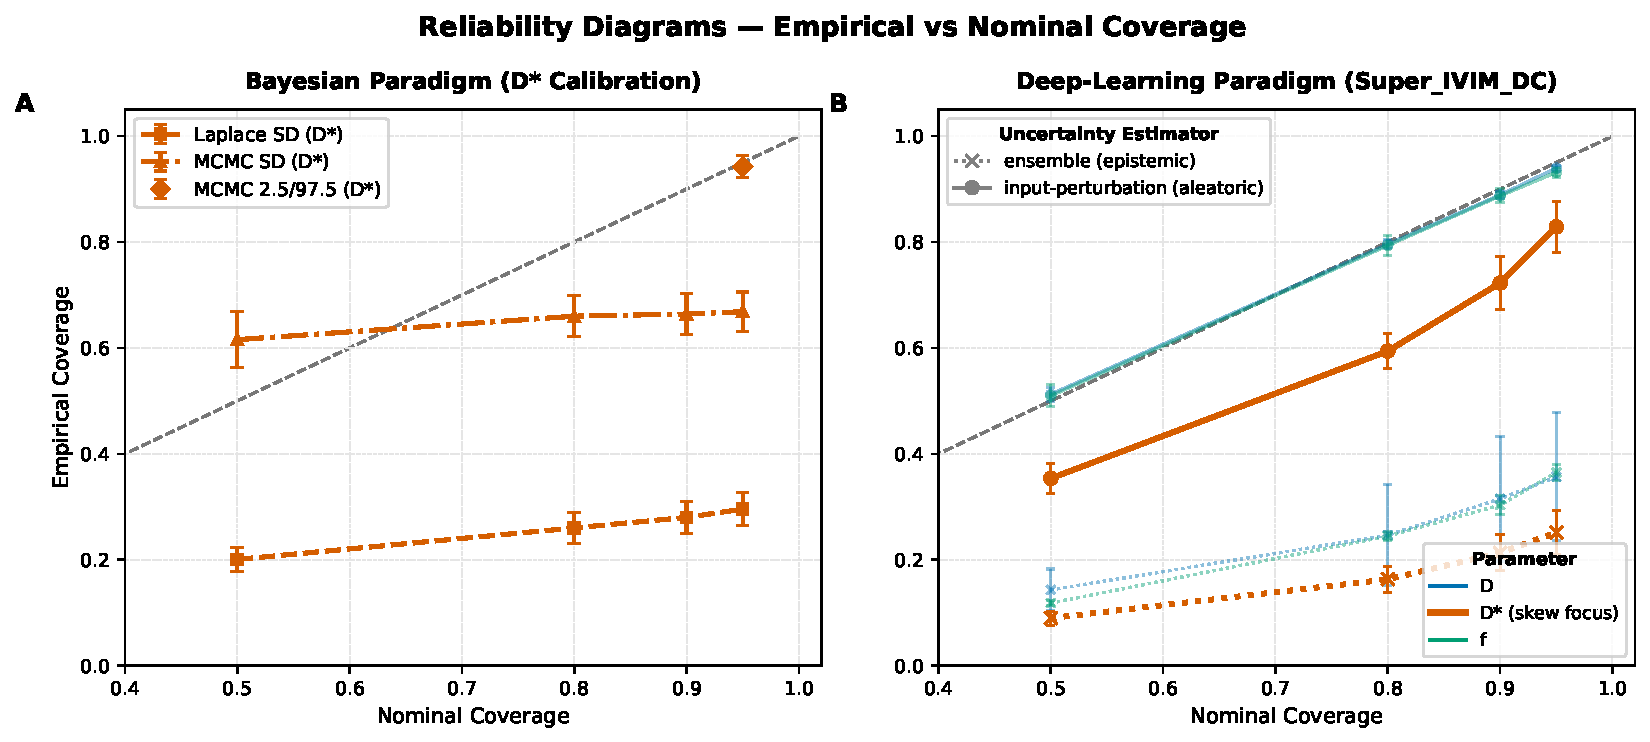
\includegraphics[width=\textwidth]{fig1_reliability_diagrams.pdf}
\caption{Reliability diagrams (predicted vs.\ empirical coverage). (A) Bayesian paradigm,
stratified by construction (Laplace, MCMC--SD, MCMC--quantile), showing \Dstar{} skew recovery
via quantile intervals. (B) Deep-learning paradigm, contrasting ensemble-over-retrains
(epistemic; severe under-coverage) and input-perturbation (predictive; matches the ceiling).
Diagonal = perfect calibration.}
\end{figure}

\begin{figure}[htbp]
\centering
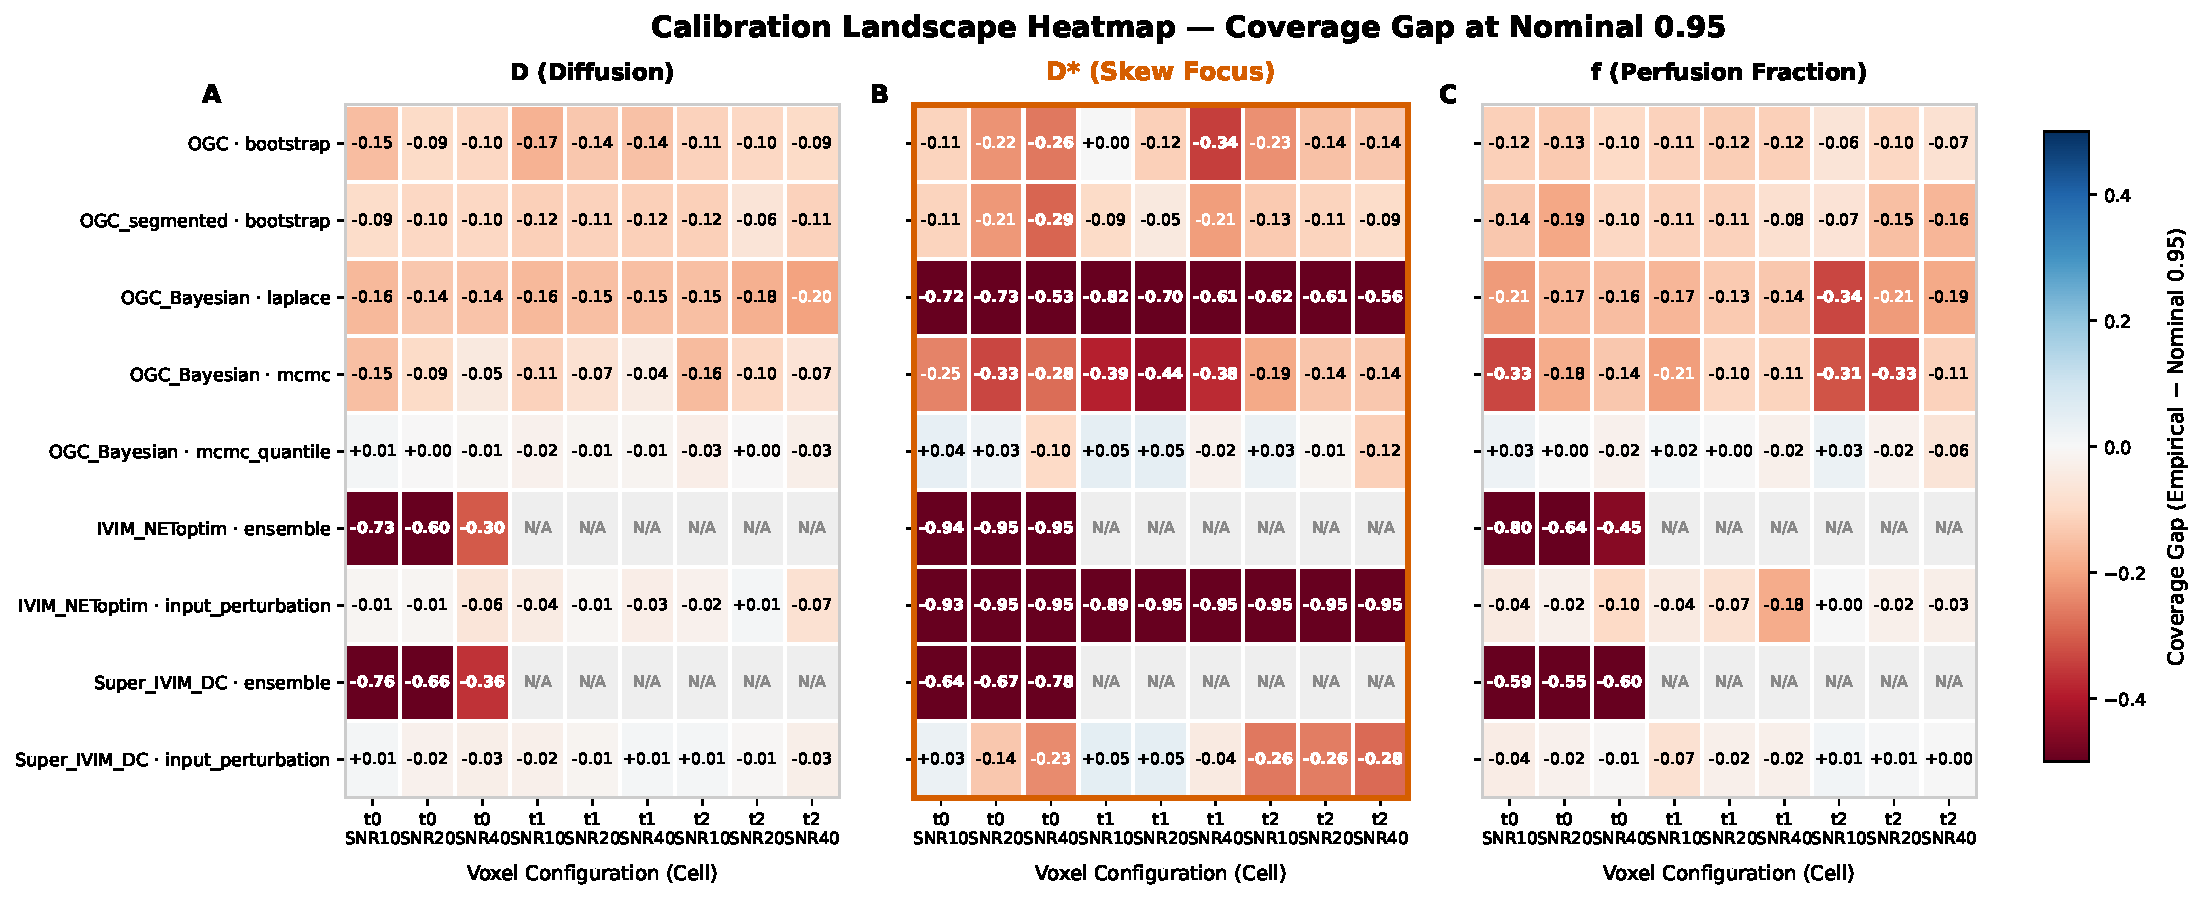
\includegraphics[width=\textwidth]{fig2_calibration_heatmap.pdf}
\caption{Calibration landscape across constructions: nine cells (three truths $\times$ three
SNR) $\times$ constructions $\times$ parameters ($D$, \Dstar{}, $f$). Color encodes coverage
gap at nominal 0.95. The \Dstar{} panel (center) is the bottleneck, recovered by quantile
intervals and input-perturbation.}
\end{figure}

\begin{figure}[htbp]
\centering
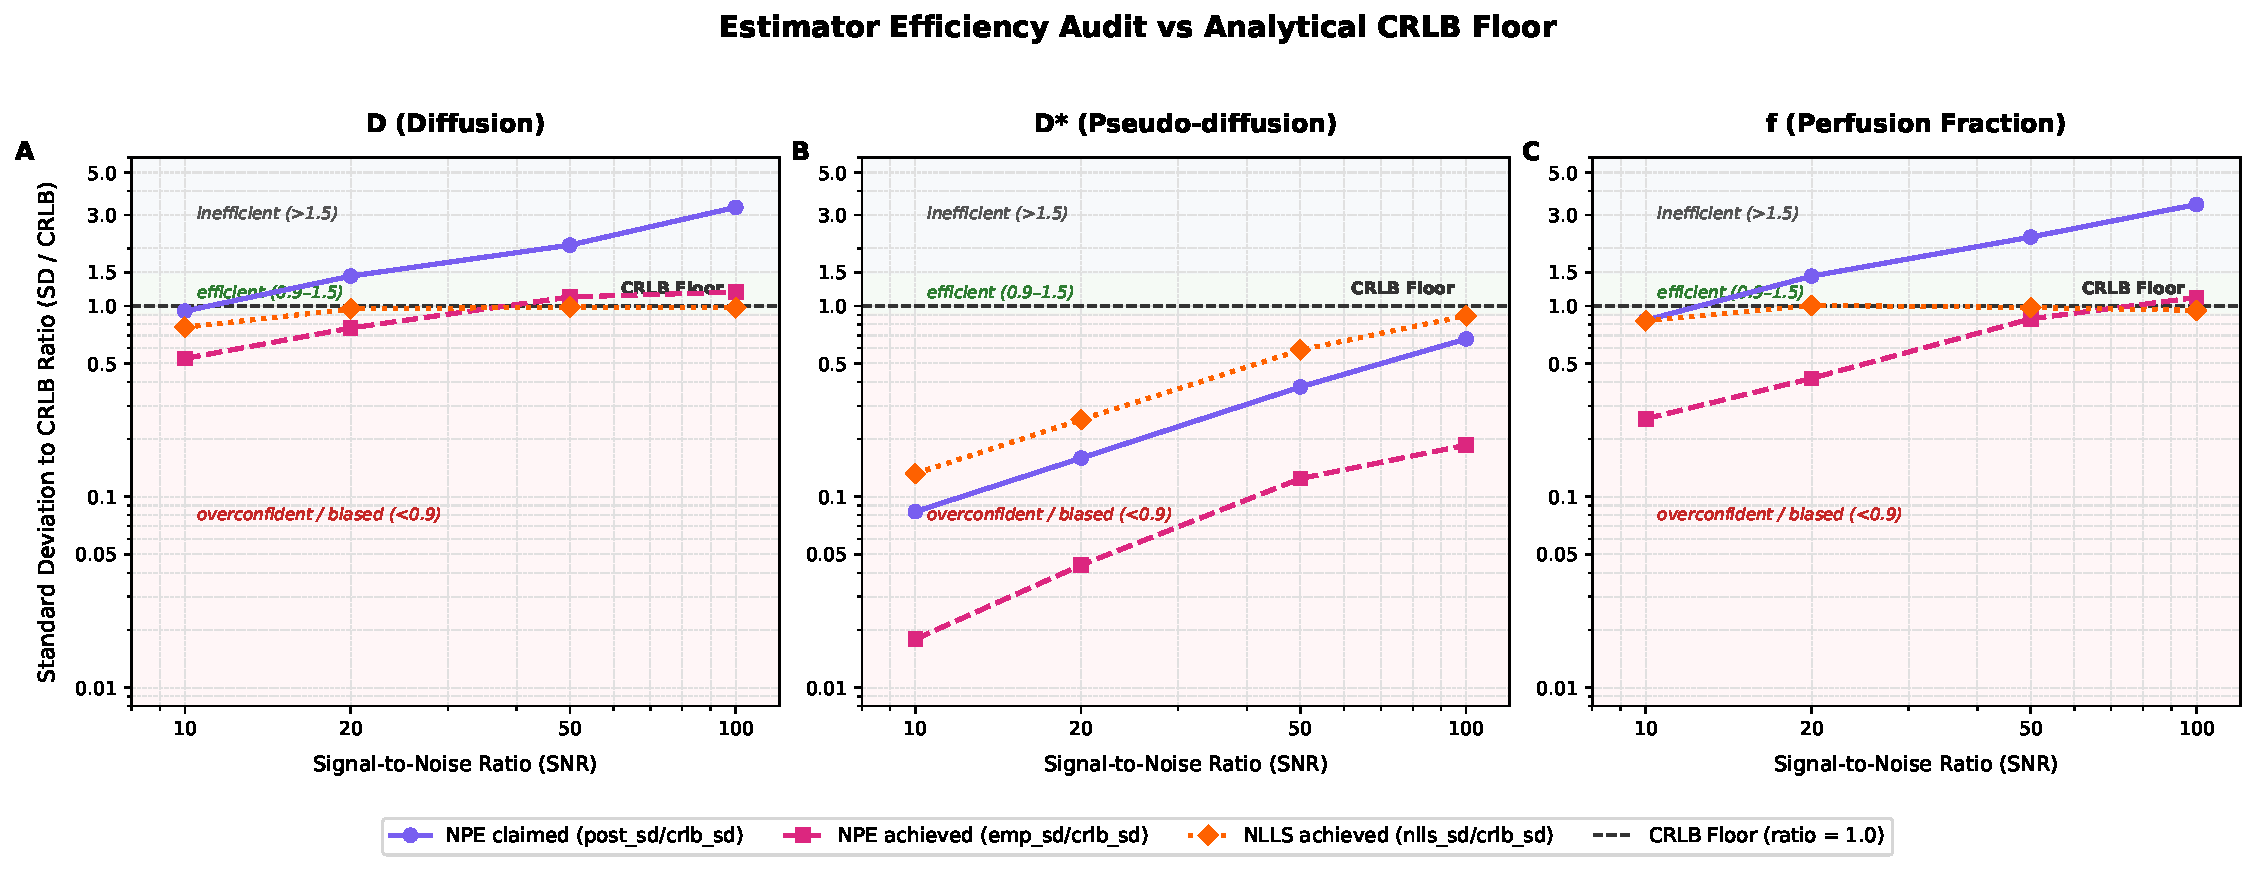
\includegraphics[width=\textwidth]{fig3_efficiency_audit.pdf}
\caption{Efficiency audit of the amortized NPE: median SD-to-CRLB ratio vs SNR for $D$,
\Dstar{}, and $f$, comparing NPE claimed posterior SD, NPE achieved empirical SD, and NLLS
achieved SD against the CRLB floor ($=1.0$). Below the floor: overconfident (claimed) or
biased (achieved); above: inefficient. \Dstar{} is overconfident and biased across SNR; $D$
and $f$ drift from near-efficient to inefficient; NLLS tracks the floor.}
\end{figure}

\begin{figure}[htbp]
\centering
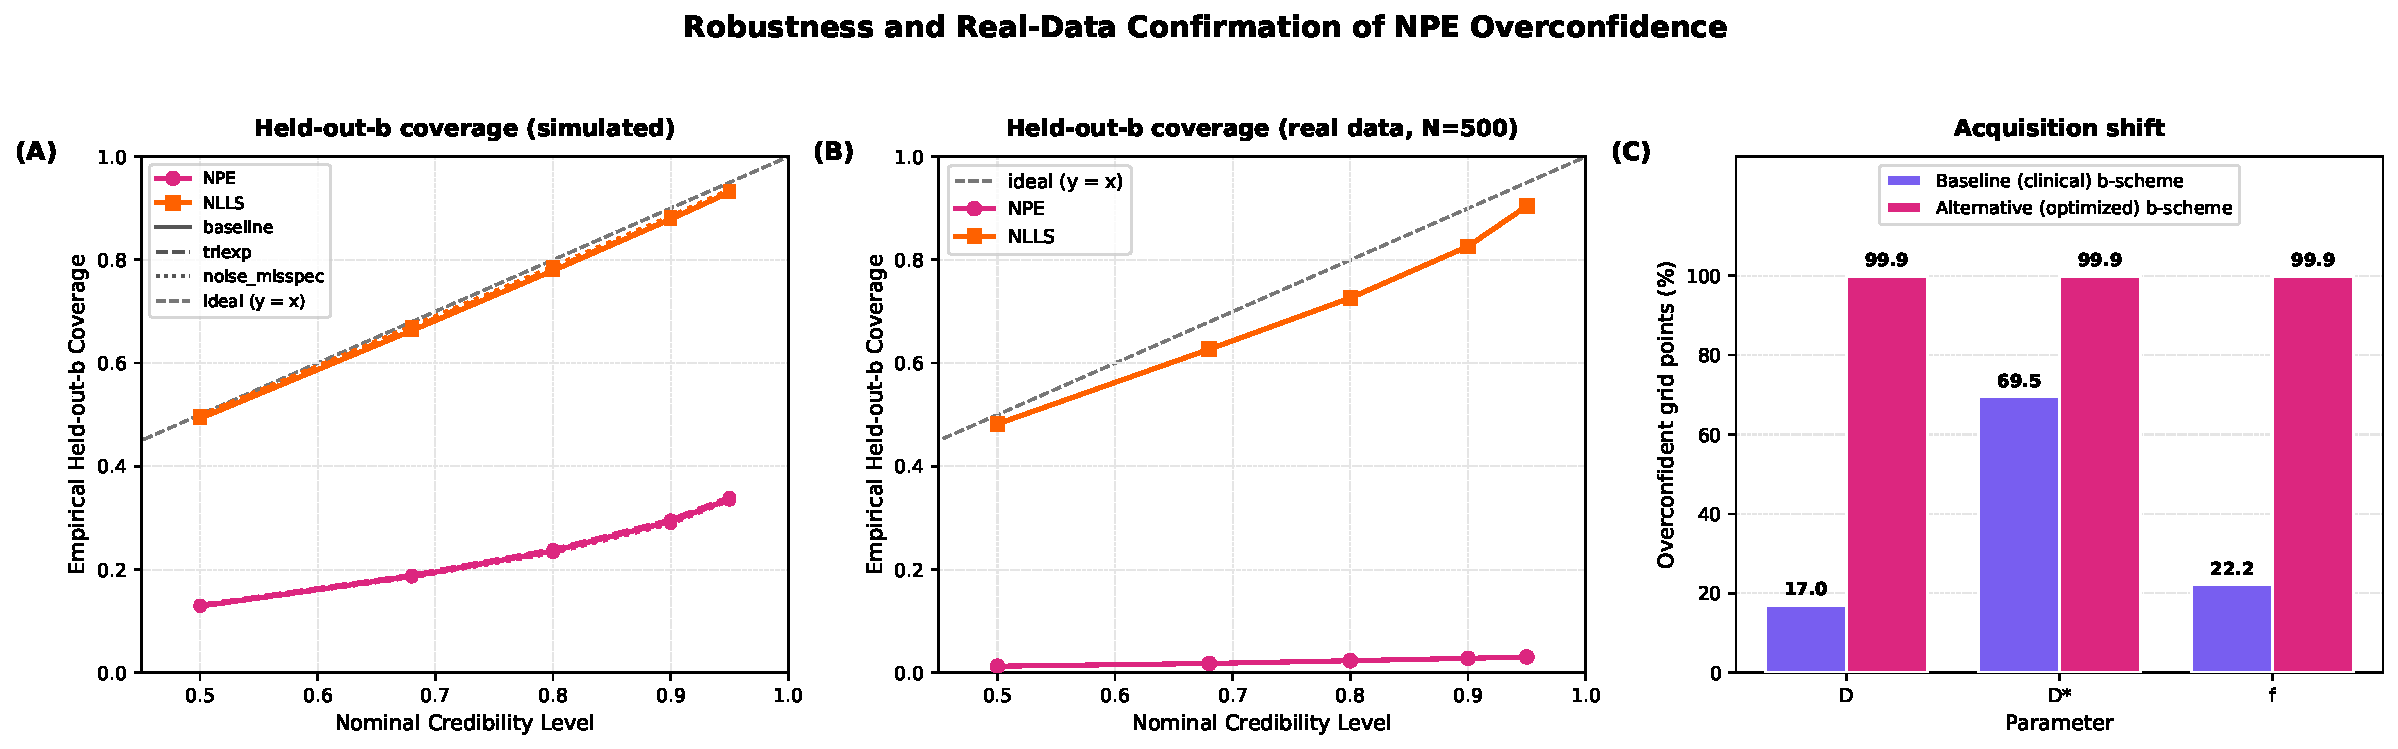
\includegraphics[width=\textwidth]{fig4_robustness.pdf}
\caption{Robustness and real-data confirmation. (A) Posterior-predictive held-out-b coverage
in simulation for NPE vs NLLS under baseline, tri-exponential, and noise-model
misspecification: the NPE under-covers by $\sim$0.61 at nominal 0.95 regardless of condition,
while NLLS stays calibrated. (B) The same check on the open multi-b in-vivo brain dataset (22)
($N=500$ voxels):
NPE coverage collapses to $\sim$0.03 at nominal 0.95. (C) Fraction of grid points
overconfident on the trained vs an alternative acquisition scheme: overconfidence rises to
$\sim$100\% off-scheme for all parameters, indicating amortized calibration does not transfer
across acquisitions.}
\end{figure}

% ======================= ACKNOWLEDGMENTS =======================
\section*{Acknowledgments}

The author acknowledges the use of a large language model (Claude Opus 4.8, Anthropic;
accessed 11 June 2026) to assist with drafting and copy-editing manuscript prose and with
writing document- and figure-generation code. All study design, analyses, numerical results,
and scientific figures were produced by the author from original data; no AI tool was used to
create, alter, or interpret research data or results. All AI-assisted text was reviewed,
revised, and approved by the author, who takes full responsibility for the accuracy and
integrity of the work.

% ======================= DATA AVAILABILITY =======================
\section*{Data Availability Statement}

All code, the calibration grid, and the efficiency map underlying this study are openly
available as a reproducibility module archived on Zenodo at
\href{https://doi.org/10.5281/zenodo.20649669}{doi:10.5281/zenodo.20649669}. The archive
contains the simulation, fitting, and amortized-NPE training and audit code; the full
calibration grid (per-cell coverage by uncertainty construction); and the CRLB efficiency
map (per-grid-point claimed, achieved, and floor SDs). The in-vivo evaluations use openly
available datasets, cited in Methods. The module is additionally offered to the OSIPI
initiative for benchmarking future IVIM uncertainty methods. No new patient data were
generated by this study.

% ======================= REFERENCES =======================
\begin{thebibliography}{99}
\setlength{\itemsep}{2pt}

\bibitem{lebihan1988} Le Bihan D, Breton E, Lallemand D, Aubin ML, Vignaud J, Laval-Jeantet M.
Separation of diffusion and perfusion in intravoxel incoherent motion MR imaging. Radiology.
1988;168(2):497-505.

\bibitem{koh2011} Koh DM, Collins DJ, Orton MR. Intravoxel incoherent motion in body
diffusion-weighted MRI: reality and challenges. AJR Am J Roentgenol. 2011;196(6):1351-1361.

\bibitem{gurneychampion2018} Gurney-Champion OJ, Klaassen R, Froeling M, et al. Comparison of
six fit algorithms for the intravoxel incoherent motion model of diffusion-weighted MRI data
of pancreatic cancer patients. PLoS One. 2018;13(4):e0194590.

\bibitem{lemke2011} Lemke A, Stieltjes B, Schad LR, Laun FB. Toward an optimal distribution of
b values for intravoxel incoherent motion imaging. Magn Reson Imaging. 2011;29(6):766-776.

\bibitem{federau2012} Federau C, Maeder P, O'Brien K, Browaeys P, Meuli R, Hagmann P.
Quantitative measurement of brain perfusion with intravoxel incoherent motion MR imaging.
Radiology. 2012;265(3):874-881.

\bibitem{while2017} While PT. A comparative simulation study of Bayesian fitting approaches to
intravoxel incoherent motion modeling in diffusion-weighted MRI. Magn Reson Med.
2017;78(6):2373-2387.

\bibitem{kaandorp2021} Kaandorp MP, Barbieri S, Klaassen R, et al. Improved unsupervised
physics-informed deep learning for intravoxel incoherent motion modeling and evaluation in
pancreatic cancer patients. Magn Reson Med. 2021;86(4):2250-2265.

\bibitem{efron1993} Efron B, Tibshirani RJ. An Introduction to the Bootstrap. New York:
Chapman and Hall; 1993.

\bibitem{orton2014} Orton MR, Collins DJ, Koh DM, Leach MO. Improved intravoxel incoherent
motion analysis of diffusion-weighted imaging by data-driven Bayesian modeling. Magn Reson
Med. 2014;71(1):411-420.

\bibitem{meeus2017} Meeus EM, Novak J, Withey SB, Zarinabad N, Dehghani H, Peet AC. Evaluation
of intravoxel incoherent motion fitting methods in low-perfused tissue. J Magn Reson Imaging.
2017;45:1325-1334.

\bibitem{cranmer2020} Cranmer K, Brehmer J, Louppe G. The frontier of simulation-based
inference. Proc Natl Acad Sci USA. 2020;117(48):30055-30062.

\bibitem{papamakarios2021} Papamakarios G, Nalisnick E, Rezende DJ, Mohamed S, Lakshminarayanan
B. Normalizing flows for probabilistic modeling and inference. J Mach Learn Res.
2021;22(57):1-64.

\bibitem{talts2018} Talts S, Betancourt M, Simpson D, Vehtari A, Gelman A. Validating Bayesian
inference algorithms with simulation-based calibration. arXiv:1804.06788. 2018.

\bibitem{lakshminarayanan2017} Lakshminarayanan B, Pritzel A, Blundell C. Simple and scalable
predictive uncertainty estimation using deep ensembles. In: Advances in Neural Information
Processing Systems (NeurIPS). 2017.

\bibitem{kendall2017} Kendall A, Gal Y. What uncertainties do we need in Bayesian deep learning
for computer vision? In: Advances in Neural Information Processing Systems (NeurIPS). 2017.

\bibitem{barbieri2020} Barbieri S, Gurney-Champion OJ, Klaassen R, Thoeny HC. Deep learning how
to fit an intravoxel incoherent motion model to diffusion-weighted MRI. Magn Reson Med.
2020;83(1):312-321.

\bibitem{korngut2022} Korngut N, Rotman E, Afacan O, et al. SUPER-IVIM-DC: intra-voxel
incoherent motion based fetal lung maturity assessment from limited DWI data using supervised
learning coupled with data-consistency. In: Medical Image Computing and Computer Assisted
Intervention (MICCAI) 2022. Lecture Notes in Computer Science. Springer; 2022.
doi:10.1007/978-3-031-16434-7\_71.

\bibitem{zhang2019} Zhang L, Vishnevskiy V, Jakab A, Goksel O. Implicit modeling with
uncertainty estimation for intravoxel incoherent motion imaging. In: IEEE 16th International
Symposium on Biomedical Imaging (ISBI). 2019:1003-1007.

\bibitem{casali2026} Casali N, Brusaferri A, Baselli G, et al. A comprehensive framework for
uncertainty quantification of voxel-wise supervised deep learning models in IVIM MRI. NMR
Biomed. 2026. doi:10.1002/nbm.70227.

\bibitem{jallais2024} Jallais M, Palombo M. Introducing $\mu$GUIDE for quantitative imaging via
generalized uncertainty-driven inference using deep learning. eLife. 2024;13:RP101069.
doi:10.7554/eLife.101069.

\bibitem{manzanopatron2025} Manzano-Patr\'on JP, Deistler M, Schr\"oder C, et al. Uncertainty
mapping and probabilistic tractography using simulation-based inference in diffusion MRI: a
comparison with classical Bayes. Med Image Anal. 2025;103:103580.
doi:10.1016/j.media.2025.103580.

\bibitem{osipidata2025} Gurney-Champion O, Rashid I, van der Thiel M, Kuppens D, Voorter P, van
Houdt P, Peterson E, Jalnefjord O. Data for the OSIPI TF2.4 IVIM-MRI Code Collection (in-vivo
brain and abdominal diffusion-weighted acquisitions). Zenodo; 2025.
doi:10.5281/zenodo.14605039.

\end{thebibliography}

\end{document}
